\documentclass[10pt]{article}
% \usepackage{geometry}
% \geometry{margin=0.2in}
\usepackage[utf8]{inputenc}

\nonstopmode
% \usepackage{minted}[cache=false]
\usepackage{graphicx} % Required for including pictures
\usepackage[figurename=Figure]{caption}
% \usepackage{float}    % For tables and other floats
\usepackage{amsmath}  % For math
\usepackage{amssymb}  % For more math
\usepackage{fullpage} % Set margins and place page numbers at bottom center
% \usepackage{paralist} % paragraph spacing
% \usepackage{subfig}   % For subfigures
%\usepackage{physics}  % for simplified dv, and 
% \usepackage{enumitem} % useful for itemization
% \usepackage{siunitx}  % standardization of si units
\usepackage{hyperref}
% \usepackage{mmacells}
% \usepackage{listings}
% \usepackage{svg}
% \usepackage{xcolor, soul}
\usepackage{bm}
\usepackage{braket}
% \usepackage{cancel}
% \usepackage{setspace}
% \usepackage{listings}
% \usepackage{listings}
% \usepackage[autoload=true]{jlcode}
% \usepackage{pygmentize}

% \definecolor{cambridgeblue}{rgb}{0.64, 0.76, 0.68}

% \sethlcolor{cambridgeblue}

\usepackage[margin=1.8cm]{geometry}
\newcommand{\C}{\mathbb C}
\newcommand{\D}{\bm D}
\newcommand{\R}{\mathbb R}
\newcommand{\Q}{\mathbb Q}
\newcommand{\Z}{\mathbb Z}
\newcommand{\N}{\mathbb N}
\newcommand{\PP}{\mathbb P}
\newcommand{\A}{\mathbb A}
\newcommand{\F}{\mathbb F}
\newcommand{\1}{\mathbf 1}
\newcommand{\ip}[1]{\left\langle #1 \right\rangle}
\newcommand{\abs}[1]{\left| #1 \right|}
\newcommand{\norm}[1]{\left\| #1 \right\|}

\def\Tr{{\rm Tr}}
\def\tr{{\rm tr}}
\def\Var{{\rm Var}}
\def\calA{{\mathcal A}}
\def\calB{{\mathcal B}}
\def\calD{{\mathcal D}}
\def\calE{{\mathcal E}}
\def\calG{{\mathcal G}}
\def\from{{:}}
\def\lspan{{\rm span}}
\def\lrank{{\rm rank}}
\def\bd{{\rm bd}}
\def\acc{{\rm acc}}
\def\cl{{\rm cl}}
\def\sint{{\rm int}}
\def\ext{{\rm ext}}
\def\lnullity{{\rm nullity}}
% \DeclareSIUnit\clight{\text{\ensuremath{c}}}
% \DeclareSIUnit\fm{\femto\m}
% \DeclareSIUnit\hplanck{\text{\ensuremath{h}}}


% \lstdefinelanguage{julia}%
%   {morekeywords={abstract,break,case,catch,const,continue,do,else,elseif,%
%       end,export,false,for,function,immutable,import,importall,if,in,%
%       macro,module,otherwise,quote,return,switch,true,try,type,typealias,%
%       using,while},%
%    sensitive=true,%
% %    alsoother={$},%
%    morecomment=[l]\#,%
%    morecomment=[n]{\#=}{=\#},%
%    morestring=[s]{"}{"},%
%    morestring=[m]{'}{'},%
% }[keywords,comments,strings]%

% \lstset{%
%     language         = Julia,
%     basicstyle       = \ttfamily,
%     keywordstyle     = \bfseries\color{blue},
%     stringstyle      = \color{magenta},
%     commentstyle     = \color{ForestGreen},
%     showstringspaces = false,
% }

% $
\begin{document}
\begin{center}
	\hrule
	\vspace{.4cm}
	{\textbf { \large CAS PY 452 --- Quantum Physics II}}
\end{center}
Emmy Blumenthal \hspace{\fill} \hspace{\fill}  \textbf{} Discussion Notes\  \\
\textbf{Date:}\  Nov 9, 2022   \hspace{\fill} \textbf{Email:}\ emmyb320@bu.edu
 
\vspace{.4cm}
\hrule

\section*{WKB wave-function and energies for the `quantum bouncing ball'}


\paragraph{Problem:}

Consider the `quantum bouncing ball.' That is, consider the single-particle system governed by the Hamiltonian, $\hat H = \frac{\hat p^2}{2m} + V(x)$, where the potential is,
\begin{align}
	V(x) = \begin{cases}
		m g x & x> 0\\
		\infty  & x \leq 0,
	\end{cases}
\end{align}
where $g>0$.
Find the WKB-approximation for the energies and wave-function.
Make a plot of the wave-function and compare to the analytical solution.

\paragraph{Solution:}

First, we find the WKB-approximated energy.
The semi-classical momentum when $x> 0$ is $p(x) = \sqrt{2m(E - mgx)}$.
There is a turning point at $x_1=0$ because $V(0) \to \infty$.
The other turning points occurs when,
\begin{align}
	p(x_2) = 0 \implies 
	x_2 = E/mg.
\end{align}
The Bohr-Sommerfeld quantization condition is,
\begin{gather}
	\int_0^{x_2} p(x) \,\mathrm{d} x
	=
	\left(
		n - \frac{1}{4}
	\right)\pi \hbar
	\implies
	\sqrt{2m}
	\int_0^{E/mg}
	\sqrt{E - m g x}
	\,\mathrm{d} x
	=
	-
	\frac{1}{gm}
	\sqrt{2m}
	\int_{E}^{0}
	\sqrt{u}
	\,\mathrm{d} u
	=
	\frac{2\sqrt{2}}{3g\sqrt{m}} E^{3/2}
	=
	\left(
		n - \frac{1}{4}
	\right) \pi \hbar\nonumber
	\\
	E_n = 
	\left(
		\frac{3\pi}{8\sqrt{2}}  \hbar g
		(4n-1)
	\right)^{2/3}
	% \implies 
	% E_4 = 
	% \left(
	% 	\frac{45\pi}{8\sqrt{2}} \hbar g
	% % \right)^{3/2}.
\end{gather}
To find the wave-function, we follow Griffiths section 9.2.
In the classically-allowed region (region I) ($E_n > V(x)$), the wave-function is,
\begin{align}
	\psi_\mathrm{I}(x) =
	\frac{A}{[2m(E_n - V(x))]^{1/4}}
	\sin(\int_x^{x_2} \sqrt{2m (E_n - V(x'))} \,\mathrm{d} x' + \pi/4).
\end{align}
We are free to add the factor of $\pi/4$ as a constant of integration; similarly, we chose the limit of integration $x_2$ arbitrarily.
We choose a sine function with this phase-factor here because it will match the asymptotic expansions of the Airy functions.
% We chose a sine function here because we need $\psi_\mathrm{I}(0) = 0$ to satisfy boundary conditions.
In the classically-disallowed region (region III) ($V(x) > E_n$),
\begin{align}
	\psi_\mathrm{III}(x)
	=
	\frac{B}{[2m(V(x) - E_n)]^{1/4}}
	\exp(-\int_{x_2}^x \sqrt{2m(V(x') - E_n)} \,\mathrm{d} x').
\end{align}
We need to deal with the `patching' region (region II) next.
We linearize the potential near the turning point: $V(x) \approx V(x_2) + (x-x_2) V'(x_2)
=
E_n + (x-x_2) V'(x_2)
$.
In this particular case, the approximation is exact because the potential is linear.
Near the turning point, we want to solve the TISE:
\begin{align}
	-\frac{\hbar^2}{2m}
	\frac{d^2\psi}{\,\mathrm{d} x^2}
	+
	(E_n + (x-x_2)V'(x_2))
	\psi
	=
	E_n \psi
	\implies 
	\frac{\hbar^2}{2m V'(x_2)}
	\frac{d^2\psi}{\,\mathrm{d} x^2}
	=
	% V'(x_2)
	(x-x_2)
	\psi.
\end{align}
By changing variables $\xi = (x-x_2)\alpha$, where $\alpha =[ 2mV'(x_2)/\hbar^2]^{1/3}$, this becomes,
\begin{align}
	\frac{d^2 \psi}{d\xi^2} = \xi \psi(\xi),
\end{align}
which has solutions $\psi = C\mathrm{Ai}(\xi) + D \mathrm{Bi}(\xi)$.

% By changing variables $\xi = (x-x_2)/\alpha$, where $\alpha = \sqrt{\hbar^2/(2m V'(x_2))}$,
% this becomes,
% \begin{align}
% 	\frac{d^2\psi}{d\xi^2}
% 	=
% 	\xi \psi(\xi),
% \end{align}
% which is Airy's equation which has solutions $\psi = C \mathrm{Ai}(\xi) + D \mathrm{Bi}(\xi)$.
The large positive $\xi$ (i.e., $x \gg x_2$) asymptotic expansion is,
\begin{align}
	\mathrm{Ai}(\xi)
	% =
	\sim
	\frac{e^{-\frac{2 \xi ^{3/2}}{3}}}{2 (\pi^2 \xi)^{1/4}},
	\qquad
	\mathrm{Bi}(\xi)
	% =
	\sim
	\frac{e^{\frac{2 \xi ^{3/2}}{3}}}{(\pi^2\xi)^{1/4}}.
\end{align}
To match to $\psi_{\mathrm{III}}(x)$, we must have $D = 0$ and,
\begin{align}
	\frac{C}{2(\pi^2 \xi)^{1/4}}
	=
	\frac{B}{(2m(V(x)- E_n))^{1/4}}.
\end{align}
The large negative $\xi$ asymptotic expansion is,
\begin{align}
	\mathrm{Ai}(\xi)
	\sim 
	\frac{1}{\sqrt{\pi}(-\xi)^{1/4}}
	\sin(\frac{2}{3}(-\xi)^{3/2} + \pi/4).
\end{align}
This means that,
\begin{align}
	\frac{C}{\sqrt{\pi}(-\xi)^{1/4}}
	=
	\frac{A}{(2m(E_n - V(x)))^{1/4}},
\end{align}
which gives us the relation between $A,B,C$.
Specifically, it gives us $A/C$ and $B/C$ so that there is only one common constant: $C$, which is determined by normalization.
Using all this, we can deduce the wave-function, but we have to choose the size of the `patching region.'
Note that the Bohr-Sommerfeld quantization condition for one `vertical wall' was derived by requiring $\psi_I(0) = 0$, so we have already implicitly taken care of boundary conditions.
The rest of the plotting and computation is continued in the attached {\em Mathematica} notebook.
See figure 1 for the results.
\begin{figure}[h!]
	\centering
	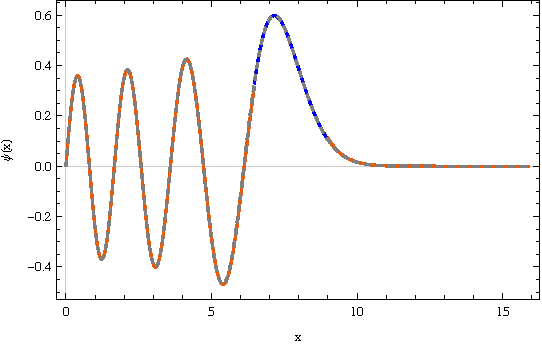
\includegraphics[width=0.8\linewidth]{fig/plot.pdf}
	\caption{
		WKB compared to exact solution.
		Here, we show the exact solution using the gray-dotted line.
		The orange line represents the wave-function in region I and III.
		The blue line represents the patching region in region II.
		We see that are able to almost exactly replicate the exact solution.
	}
\end{figure}


\section*{The general (and numerical) approach to finding WKB energies}

If we want to find WKB estimations for the energies, we need to solve the Bohr-Sommerfeld quantization condition for the energies.
The process goes like this:

\paragraph{Write the semi-classical momentum $p(x,E) = \sqrt{2m[E - V(x)]}$.}
Here, we explicitly write the energy $E$ as part of the momentum to remind us that we do not yet know the energy.

\paragraph{Find the turning points.}
The turning points occur when $E = V(x)$ or equivalently $p(x,E) = 0$.
This equation implicitly defines turning points $x_1(E)$ and $x_2(E)$ (where $x_1(E) < x_2(E)$) in terms of the so-far-unknown energy.
If there are vertical walls within the range of the relevant $E$, one or both of these turning points might be trivial (i.e., at the vertical wall).
% Note that there is a possibility that after a certain energy level, you might have to change from the case without vertical walls to the case with vertical walls.

\paragraph{Identify and solve the Bohr-Sommerfeld quantization condition.}
To obtain the $n$th energy (starting at $n=1$), we solve the equation:
\begin{align}
	\int_{x_1(E_n)}^{x_2(E_n)}
	p(x',E_n) \,\mathrm{d} x'
	=
	\pi \hbar (n - \phi),
\end{align}
where $\phi = 0$ for two vertical walls at energy $E$, $\phi = \frac{1}{4}$ for one vertical wall at energy $E$, and $\phi = \frac{1}{2}$ for no vertical walls.
This equation implicitly defines $E_n$.


\section*{A reminder on exact diagonalization}

Solving the dynamics and behavior of a quantum mechanical system in many cases reduces to solving the time-independent Schrodinger equation,

\begin{align}
E \psi(x) = - \frac{\hbar^2}{2m} \frac{d^2\psi}{\,\mathrm{d} x^2} + V(x) \psi(x).
\end{align}
At heart, this is solving the eigenvalue/eigenvector problem $E\psi(x) = \hat H \psi(x)$.
In general, this problem is very tricky because we are trying to find closed-form expressions for eigenfunctions.
However, if $\hat H$ can be represented as a matrix, this problem is less tricky and more systematic as there are algorithms that efficiently and accuractely diagonalize any matrix over the complex numbers.

Our strategy to turn the continuum problem into a matrix eigenvalue/eigenvector problem is to discretize space with some points $x_1,x_2,\dots,x_n,\dots,x_N$ and find stationary states at these points.
In the world of scientific computing, these points are sometimes called a 'stencil'.
We take these points to be seperated by some uniform spacing $\Delta x$; we are discovering an interval of total length $L = N\Delta x$.
For now, we assume that there are fixed boundary conditions, meaning that all values beyond $x_N$ or before $x_1$ are all zero.
We denote a state entirely located at a point $x_i$ with $\ket{x_i}$. 
In the basis $\beta = \{\ket{x_1},\ket{x_2},\dots,\ket{x_N}\}$,
\begin{align}
\ket{\psi_n}_\beta
=
\begin{bmatrix}
\psi_n(x_1)\\
\psi_n(x_2)\\
\vdots\\
\psi_n(x_i)\\
\vdots\\
\psi_n(x_N)\\
\end{bmatrix}.
\end{align}
When we discretize like this, operators are now  matrices!
For example, in the position basis, the position operator is:
\begin{align}
\hat x_\beta
=
\begin{bmatrix}
x_1 & 0 & 0  & \cdots &0 & 0 & 0 \\
0 & x_2 & 0 & \cdots &0 & 0 & 0\\
0 & 0 & x_3 & \cdots & 0 & 0 & 0\\
\vdots & \vdots & \vdots & \ddots & \vdots & \vdots & \vdots\\
0 & 0 & 0 & \cdots & x_{N-2} & 0&0\\
0 & 0 & 0 & \cdots & 0 & x_{N-2} & 0\\
0 & 0 & 0 & \cdots & 0 & 0& x_{N}\\
\end{bmatrix}
\end{align}
This makes the potential operator,
\begin{align}
V(\hat x)_\beta
=
\begin{bmatrix}
V(x_1) & 0 & 0  & \cdots &0 & 0 & 0 \\
0 & V(x_2) & 0 & \cdots &0 & 0 & 0\\
0 & 0 & V(x_3) & \cdots & 0 & 0 & 0\\
\vdots & \vdots & \vdots & \ddots & \vdots & \vdots & \vdots\\
0 & 0 & 0 & \cdots & V(x_{N-2}) & 0&0\\
0 & 0 & 0 & \cdots & 0 & V(x_{N-2}) & 0\\
0 & 0 & 0 & \cdots & 0 & 0& V(x_{N})\\
\end{bmatrix}
\end{align}
Using the central difference formula for the first derivative,
\begin{align}
\frac{df}{\,\mathrm{d} x}
=
\lim_{h\to 0}
\frac{f(x+h) -f(x-h)}{2h},
\end{align}
we can write the dertivative operator as,
\begin{align}
\frac{d}{\,\mathrm{d} x}
=
\frac{1}{2\Delta x}
\begin{bmatrix}
0 & 1 & 0  & \cdots &0 & 0 & 0 \\
-1 & 0 & 1 & \cdots &0 & 0 & 0\\
0 & -1 & 0 & \cdots & 0 & 0 & 0\\
\vdots & \vdots & \vdots & \ddots & \vdots & \vdots & \vdots\\
0 & 0 & 0 & \cdots & 0 & 1 & 0\\
0 & 0 & 0 & \cdots & -1 & 0 & 1\\
0 & 0 & 0 & \cdots & 0 & -1 & 0\\
\end{bmatrix}.
\end{align}
This makes the momentum operator:
\begin{align}
\hat p_\beta
=
- i \hbar \frac{d}{\,\mathrm{d} x}
=
\frac{-i\hbar}{2\Delta x}
\begin{bmatrix}
0 & 1 & 0  & \cdots &0 & 0 & 0 \\
-1 & 0 & 1 & \cdots &0 & 0 & 0\\
0 & -1 & 0 & \cdots & 0 & 0 & 0\\
\vdots & \vdots & \vdots & \ddots & \vdots & \vdots & \vdots\\
0 & 0 & 0 & \cdots & 0 & 1 & 0\\
0 & 0 & 0 & \cdots & -1 & 0 & 1\\
0 & 0 & 0 & \cdots & 0 & -1 & 0\\
\end{bmatrix}.
\end{align}
The second derivative of a one-dimensional function can be written as,
\begin{align}
\frac{d^2f}{\,\mathrm{d} x^2}
=
\lim_{h\to 0}
\frac{f(x+h) - 2f(x)+f(x-h)}{h^2},
\end{align}
so we can form a second derivative operator, sometimes called the discete Laplacian, $\Delta$:
\begin{align}
\frac{d^2}{\,\mathrm{d} x^2} 
= \Delta
=
\frac{1}{\Delta x^2}
\begin{bmatrix}
-2 & 1 & 0  & \cdots &0 & 0 & 0 \\
1 & -2 & 1 & \cdots &0 & 0 & 0\\
0 & 1 & -2 & \cdots & 0 & 0 & 0\\
\vdots & \vdots & \vdots & \ddots & \vdots & \vdots & \vdots\\
0 & 0 & 0 & \cdots & -2 & 1 & 0\\
0 & 0 & 0 & \cdots & 1 & -2 & 1\\
0 & 0 & 0 & \cdots & 0 & 1 & -2\\
\end{bmatrix}.
\end{align}
With all this, we can write the Hamiltonian operator as a sum of matrices!

It is also important to touch on normalization.
In order to be consistent with the continuous case, we want to normalize our states such that,
\begin{align}
	\int \mathrm{d} x\, \psi_n^\ast(x)\psi_n(x)
	= 1
	\implies
	\sum_{i=1}^N
	\psi_n^\ast(x_i)\psi_n(x_i) \Delta x = 1,
\end{align}
which is consistent with the definition of the Riemann integral.
This could be equivalently stated as,
\begin{align}
	\ket{\psi_n}_\beta^\dagger
	\ket{\psi_n}_\beta
	=
	\frac{1}{\Delta x},
\end{align}
where considering $\ket{\psi_n}_\beta$ as a column vector.




\end{document}






